\chapter{Tương quan Ising, trường trung bình và từ hóa tự phát}

\lectureoverview{Chuỗi Ising một chiều có thể được giải chính xác bằng cách thay các spin tại nút bằng các biến liên kết. Phép đổi biến đó biến hàm phân hoạch thành một tích và cho thấy mọi tương quan ở nhiệt độ hữu hạn đều suy giảm theo hàm mũ. Các mạng ở số chiều cao hơn ứng xử khác vì mỗi spin nhận ảnh hưởng từ nhiều láng giềng. Xem ảnh hưởng tổng hợp của chúng như một trường trung bình sẽ cho một phương trình tự nhất quán, một nhiệt độ tới hạn kiểu trường trung bình, và một mô tả chính xác về cách một trường ngoài nhỏ tùy ý chọn ra một pha có từ hóa.}

\section{Điều Ising thực sự đã tìm ra}

Điểm lịch sử này cần được phát biểu cho chính xác. Ernst Ising đã giải mô hình một chiều do Wilhelm Lenz giao và tìm ra đúng rằng không có chuyển pha ở nhiệt độ hữu hạn. Điều đi quá xa là suy ra rằng cùng kết luận ấy phải đúng ở mọi số chiều. Không phải vậy. Mô hình hai chiều đã có một pha có trật tự ở nhiệt độ thấp.

Một nghiệm chính xác ở số chiều cao hơn là quá tham vọng đối với mục đích hiện tại. Một phép gần đúng minh bạch về mặt vật lý là đủ để chỉ ra chuyển pha khi mỗi spin có nhiều láng giềng. Tuy nhiên, trước khi thực hiện phép gần đúng đó, rất đáng để giải chính xác chuỗi một chiều. Sự tương phản giữa đáp án chính xác của một chiều và phép gần đúng ở số chiều cao xác định cơ chế mà một chiều còn thiếu.

Ở đây, chuyển pha có nghĩa nhiều hơn sự tăng cường dần dần của một xu hướng ưu tiên vốn đã có. Khi nhiệt độ đi qua một giá trị tới hạn, trạng thái cân bằng thu được một tính chất vĩ mô mới: một độ từ hóa khác không có thể tồn tại ngay cả sau khi trường ngoài dùng để định hướng mẫu đã bị loại bỏ. Vì vậy, phép tính phải trả lời hai câu hỏi tách biệt. Một spin ở xa có nhớ hướng của một spin được chọn hay không, và một trường vô cùng nhỏ có thể sắp xếp trật tự cho một mẫu lớn tùy ý hay không?

\section{Một spin như một viên gạch cơ bản dùng lặp lại}

Xét một biến hai trạng thái
\begin{equation}
\sigma=\pm1,
\end{equation}
và chọn quy ước năng lượng
\begin{equation}
E(\sigma)=-J\sigma,
\qquad J>0.
\end{equation}
Khi đó trạng thái \(\sigma=+1\) có năng lượng thấp hơn. Tham số \(J\) có thể biểu diễn một mômen từ nhân với một trường đặt vào, nhưng trong phép tính này chỉ có tích đó đi vào.

Hãy coi spin này như một phân hệ nhỏ cân bằng nhiệt với mọi thứ còn lại. Hàm phân hoạch của nó là
\begin{align}
z
&=\sum_{\sigma=\pm1}e^{-\beta E(\sigma)}
 =\sum_{\sigma=\pm1}e^{\beta J\sigma} \\
&=e^{\beta J}+e^{-\beta J}
 =2\cosh(\beta J).
\end{align}

Cùng kết quả ấy có thể được đặt vào một tập hợp gồm \(N\) spin độc lập. Hàm phân hoạch đầy đủ khi đó đơn giản là \(Z=z^N\), nên \(\log Z=N\log z\) và mọi đại lượng nhiệt động quảng tính đều sẽ bằng \(N\) lần giá trị một-spin của nó. Cách nhìn theo phân hệ này thay cho phép đếm tổ hợp dài dòng xem có bao nhiêu spin hướng lên và hướng xuống, nhưng chứa cùng một thông tin.
Năng lượng trung bình suy ra từ đạo hàm logarit:
\begin{align}
\expect{E}
&=-\frac{\partial}{\partial\beta}\log z \\
&=-J\frac{\sinh(\beta J)}{\cosh(\beta J)}
 =-J\tanh(\beta J).
\end{align}
Vì \(E=-J\sigma\),
\begin{equation}
\expect{\sigma}=\tanh(\beta J).
\end{equation}

\begin{figure}[ht]
\centering
\includegraphics[width=0.80\textwidth]{lecture_09_figure_02.png}
\caption{Năng lượng và độ từ hóa của một spin, được đưa về dạng tang hyperbol.}
\lectureframe{00:10:06}
\end{figure}

Công thức duy nhất này bao hàm cả hai giới hạn nhiệt độ. Ở nhiệt độ thấp, \(\beta J\gg1\), và spin gần như chắc chắn ở trong trạng thái năng lượng thấp hơn. Ở nhiệt độ cao, \(\beta J\ll1\), nên
\begin{equation}
\expect{\sigma}\simeq \beta J\longrightarrow0.
\end{equation}
Dao động nhiệt xóa đi sự thiên lệch năng lượng.

\begin{classroomqa}
\audiencequestion{Năng lượng trung bình có phải mang dấu trừ không?}
\lecturerresponse{Có. Đồng nhất thức nhiệt động là \(\expect{E}=-\partial_\beta\log z\), nên kết quả là \(-J\tanh(\beta J)\). Chia cho thừa số \(-J\) trong \(E=-J\sigma\) khi đó cho độ từ hóa dương \(\expect{\sigma}=\tanh(\beta J)\). \lecturetimestamp{00:09:15--00:09:44}}
\end{classroomqa}

\section{Chuỗi một chiều}

Đặt \(N\) spin trên một chuỗi hở và cho các spin lân cận tương tác:
\begin{equation}
H=-J\sum_{i=1}^{N-1}\sigma_i\sigma_{i+1},
\qquad \sigma_i=\pm1.
\label{eq:ising-chain}
\end{equation}
Với \(J>0\), một cặp song song đóng góp \(-J\), còn một cặp phản song song đóng góp \(+J\). Vì thế, hai trạng thái cơ bản là
\begin{equation}
(+,+,\ldots,+)
\qquad\text{and}\qquad
(-,-,\ldots,-).
\end{equation}

\begin{figure}[ht]
\centering
\includegraphics[width=0.80\textwidth]{lecture_09_figure_03.png}
\caption{Hamiltonian của chuỗi hở và tổng Boltzmann của nó.}
\lectureframe{00:19:15}
\end{figure}

Đổi \(J\) thành \(-J\) làm ưu tiên các spin xen kẽ. Trên một chuỗi hở, hoặc trên một chuỗi tuần hoàn chẵn, phép định nghĩa lại
\begin{equation}
\widetilde{\sigma}_i=(-1)^i\sigma_i
\end{equation}
đưa dấu phản sắt từ về lại dấu sắt từ. Sự khác biệt này là vật lý, nhưng phần đại số của hàm phân hoạch một chiều thì như nhau. Chuỗi tuần hoàn lẻ là ngoại lệ quen thuộc vì nó không thể xen kẽ mà không nảy sinh xung đột.

\begin{classroomqa}
\audiencequestion{Trong Hamiltonian của chuỗi có trường từ ngoài không?}
\lecturerresponse{Chưa. Phương trình~\eqref{eq:ising-chain} chỉ chứa ghép cặp láng giềng gần nhất. Một trường ngoài đều sẽ được thêm vào sau như một hạng riêng, \(-h\sum_i\sigma_i\), chính để kiểm tra trạng thái có trật tự đáp ứng thế nào trước một thiên lệch nhỏ tùy ý. \lecturetimestamp{00:18:54--00:19:13}}
\end{classroomqa}

\subsection{Ký ức như một hàm tương quan}

Giả sử biết rằng \(\sigma_i\) hướng lên. Thông tin đó có ảnh hưởng tới một spin cách \(r\) liên kết không? Đại lượng chẩn đoán là
\begin{equation}
C(r)=\expect{\sigma_i\sigma_{i+r}}.
\end{equation}
Nếu \(C(r)\) tiến tới một số khác không khi \(r\to\infty\), hệ còn giữ ký ức tầm xa. Nếu nó tiến tới 0, ảnh hưởng của spin đầu tiên rốt cuộc biến mất.

Trò truyền tin cho trực giác đúng. Mỗi người truyền một ký hiệu nhị phân cho người kế tiếp. Nếu mọi lần truyền đều hoàn hảo, bit ban đầu tồn tại mãi mãi. Nếu mỗi bước có bất kỳ xác suất sai khác không nào, sự truyền lặp đi lặp lại cuối cùng sẽ làm mất thông điệp gốc. Nhiệt độ bằng không là giới hạn truyền hoàn hảo của chuỗi Ising. Bất kỳ nhiệt độ dương nào cũng cho phép đôi lúc có bất đồng giữa các láng giềng.

Để có một hình dung định lượng, giả sử một lần truyền đơn lẻ có độ trung thực \(0.99\). Hai lần truyền hoàn hảo xảy ra với xác suất \(0.99^2=0.9801\), và mỗi bước bổ sung cung cấp thêm một thừa số \(0.99\). Một trăm bước đã khiến sai lỗi trở nên phổ biến; mười nghìn bước xóa sạch ký ức trên thực tế. Chuỗi Ising dùng một độ đo có dấu của độ trung thực chứ không phải xác suất không lỗi này, nhưng sự mất mát theo phép nhân vẫn là cùng một ý tưởng.

Sự tương tự này trở nên chính xác sau khi phân biệt xác suất với tương quan. Nếu \(p\) là xác suất để các spin kề nhau có cùng giá trị, thì
\begin{equation}
\expect{\sigma_i\sigma_{i+1}}
=p-(1-p)=2p-1.
\end{equation}
Vì vậy, đại lượng được nhân qua từng liên kết là độ phù hợp vượt mức \(2p-1\), chứ không phải bản thân \(p\).

\section{Biến liên kết và hàm phân hoạch chính xác}

Phép đổi biến mang tính quyết định là mô tả các quan hệ thay vì từng spin riêng lẻ:
\begin{equation}
\mu_i=\sigma_i\sigma_{i+1},
\qquad i=1,\ldots,N-1.
\label{eq:bond-variable}
\end{equation}
Mỗi biến liên kết bằng \(+1\) khi đồng hướng và bằng \(-1\) khi ngược hướng. Nếu spin thứ nhất được cố định, các liên kết xác định mọi spin về sau:
\begin{align}
\sigma_2&=\sigma_1\mu_1,\\
\sigma_3&=\sigma_1\mu_1\mu_2,\\
\sigma_{r+1}&=\sigma_1\prod_{k=1}^{r}\mu_k.
\end{align}
Không có dư thừa. Dữ liệu \((\sigma_1,\mu_1,\ldots,\mu_{N-1})\) tương đương với \((\sigma_1,\ldots,\sigma_N)\).

Trong các biến này, năng lượng đơn giản là
\begin{equation}
H=-J\sum_{i=1}^{N-1}\mu_i.
\end{equation}
Các biến tại nút vốn tương tác đã trở thành các biến liên kết độc lập. Lấy tổng trước trên hai giá trị của \(\sigma_1\) cho
\begin{align}
Z_N
&=2\sum_{\{\mu_i=\pm1\}}
\exp\left(\beta J\sum_{i=1}^{N-1}\mu_i\right)\\
&=2\prod_{i=1}^{N-1}
\left(\sum_{\mu_i=\pm1}e^{\beta J\mu_i}\right)\\
&=2\left[2\cosh(\beta J)\right]^{N-1}.
\label{eq:chain-partition}
\end{align}
Có \(N-1\) thừa số vì một chuỗi hở gồm \(N\) nút có \(N-1\) liên kết.

Hệ số 2 đứng đầu là do lựa chọn toàn cục của spin thứ nhất. Nó chỉ đóng góp \(\log2\) vào \(\log Z_N\), trong khi các liên kết đóng góp một hạng tỉ lệ với \(N-1\). Thừa số này quan trọng cho việc đếm chính xác ở kích thước hữu hạn nhưng biến mất khỏi mật độ năng lượng tự do khi \(N\to\infty\). Đó là lý do vì sao trên bảng có thể gọi nó là "không có gì to tát" mà không thực sự bỏ nó đi.

\begin{figure}[ht]
\centering
\includegraphics[width=0.82\textwidth]{lecture_09_figure_04.png}
\caption{Hamiltonian theo nút được viết lại thành tổng trên các liên kết độc lập và hàm phân hoạch phân tích thành tích thu được.}
\lectureframe{00:35:35}
\end{figure}

\begin{classroomqa}
\audiencequestion{Khi đáp án cuối cùng trở thành một lũy thừa, tổng ở số mũ đã đi đâu?}
\lecturerresponse{Trước khi trở thành lũy thừa, nó đã trở thành một tích:
\[
e^{\beta J\sum_i\mu_i}=\prod_i e^{\beta J\mu_i}.
\]
Khi đó, tổng trên mọi cấu hình liên kết tách thành một tổng hai hạng cho mỗi liên kết. Vì mọi thừa số đều là \(2\cosh(\beta J)\), tích là lũy thừa bậc \((N-1)\) của nó. Viết ra trường hợp ba spin và hai liên kết sẽ làm sự phân tích thành tích hoàn toàn tường minh. \lecturetimestamp{00:33:25--00:35:36}}
\end{classroomqa}

Đây là một mô tả đối ngẫu đơn giản: các biến liên kết với nhau trên các nút đã được thay bằng các biến độc lập trên các liên kết. Từ \emph{đối ngẫu} là thích hợp vì cùng một hệ có hai mô tả với các bậc tự do trông rất khác nhau. Ở đây, đó là một phép đổi biến chính xác cho một chuỗi hở một chiều.

Theo ngôn ngữ mạng, các biến ban đầu nằm trên các đỉnh còn các biến mới nằm trên các cạnh. Lựa chọn toàn cục của spin thứ nhất là mẩu dữ liệu bổ sung duy nhất cần để khôi phục các đỉnh từ các cạnh. Sự hoán đổi nút-liên kết này là một ví dụ khiêm tốn của một khuôn mẫu trở nên mạnh hơn rất nhiều trong cơ học thống kê nhiều chiều.

\subsection{Độ trung thực của láng giềng gần nhất}

Mọi liên kết đều có cùng một phân bố,
\begin{equation}
\begin{aligned}
\Pr(\mu=+1)&=\frac{e^{\beta J}}{2\cosh(\beta J)},\\
\Pr(\mu=-1)&=\frac{e^{-\beta J}}{2\cosh(\beta J)}.
\end{aligned}
\end{equation}
Do đó,
\begin{equation}
\expect{\mu_i}
=\expect{\sigma_i\sigma_{i+1}}
=\tanh(\beta J).
\label{eq:nearest-correlation}
\end{equation}

\begin{figure}[ht]
\centering
\includegraphics[width=0.80\textwidth]{lecture_09_figure_05.png}
\caption{Tương quan láng giềng gần nhất được biểu diễn như giá trị trung bình của biến liên kết.}
\lectureframe{00:36:52}
\end{figure}

Vì thế, xác suất để hai spin láng giềng cùng hướng là
\begin{equation}
p_{\rm same}
=\frac{1+\tanh(\beta J)}{2}.
\end{equation}
Nó lớn hơn một nửa khi \(J\) dương, tiến tới 1 ở nhiệt độ bằng 0, và trở thành một nửa ở nhiệt độ vô hạn.

\begin{classroomqa}
\audiencequestion{Vì sao một tương quan dương giữa các láng giềng gần nhất lại có nghĩa là các spin ưu tiên cùng hướng chứ không phải ngược hướng?}
\lecturerresponse{Với \(J>0\), một liên kết cùng hướng có năng lượng \(-J\) và một liên kết ngược hướng có năng lượng \(+J\). Giá trị dương của \(\expect{\mu}\) cho biết rằng \(\mu=+1\), tức là cùng hướng, xuất hiện thường xuyên hơn. Việc một vật liệu thực có tương tác hiệu dụng sắt từ hay phản sắt từ phụ thuộc vào cấu trúc điện tử vi mô của nó; quy ước dấu hiện tại mô tả một chất sắt từ. \lecturetimestamp{00:43:45--00:44:48}}
\end{classroomqa}

\begin{classroomqa}
\audiencequestion{Tương quan này sẽ ra sao ở nhiệt độ rất cao?}
\lecturerresponse{Khi \(T\to\infty\), \(\beta\to0\) và \(\tanh(\beta J)\to0\). Khi đó, ngay cả các láng giềng gần nhất cũng không mang thông tin gì về nhau: mỗi spin về thực chất chỉ là một phỏng đoán ngẫu nhiên. \lecturetimestamp{00:46:42--00:47:20}}
\end{classroomqa}

\subsection{Tương quan tầm xa}

Đối với các spin cách nhau \(r\) liên kết,
\begin{align}
\sigma_i\sigma_{i+r}
&=\sigma_i
\left(\prod_{k=i+1}^{i+r-1}\sigma_k^2\right)
\sigma_{i+r}\\
&=(\sigma_i\sigma_{i+1})
(\sigma_{i+1}\sigma_{i+2})\cdots
(\sigma_{i+r-1}\sigma_{i+r})\\
&=\prod_{k=i}^{i+r-1}\mu_k.
\end{align}
Vì các \(\mu_k\) độc lập,
\begin{equation}
C(r)=\expect{\sigma_i\sigma_{i+r}}
=\left[\tanh(\beta J)\right]^r.
\label{eq:exact-correlation}
\end{equation}

\begin{figure}[ht]
\centering
\includegraphics[width=0.80\textwidth]{lecture_09_figure_06.png}
\caption{Các thừa số trung gian \(\sigma_k^2=1\) biến tích của hai spin ở xa thành tích của các liên kết độc lập.}
\lectureframe{00:41:35}
\end{figure}

\begin{classroomqa}
\audiencequestion{Hàm tương quan chỉ chứa hai spin ở hai đầu. Tất cả các spin trung gian xuất hiện từ đâu?}
\lecturerresponse{Chúng chỉ được chèn vào dưới dạng các thừa số bằng một: \(\sigma_k^2=1\). Ghép các bản sao kề nhau thành cặp sẽ biến tích ở hai đầu thành các biến liên kết, đúng là những biến có phân bố nhiệt phân tích thành tích. Giá trị của hàm tương quan không hề thay đổi. \lecturetimestamp{00:41:41--00:42:26}}
\end{classroomqa}

Ở mọi nhiệt độ hữu hạn,
\begin{equation}
0<\tanh(\beta J)<1,
\end{equation}
nên ký ức suy giảm theo hàm mũ. Nếu viết
\begin{equation}
C(r)=e^{-r/\xi}
\end{equation}
thì độ dài tương quan chính xác được định nghĩa bởi
\begin{equation}
\xi^{-1}=-\log\!\left[\tanh(\beta J)\right].
\label{eq:correlation-length}
\end{equation}
Chỉ tại \(T=0\) thì \(\xi\) mới phân kỳ. Ở nhiệt độ thấp nhưng khác không,
\begin{equation}
\xi\simeq \frac{1}{2}e^{2\beta J},
\end{equation}
nên chuỗi có thể chứa những đoạn thẳng hàng rất dài mà vẫn không có trật tự tầm xa vô hạn thực sự.

Vì thế chuỗi trông như tụ thành từng cụm. Ta thấy một đoạn dài các spin hướng lên, rồi một lần đổi hướng, rồi một đoạn dài các spin hướng xuống, rồi lại một lần đổi hướng khác. Nhiệt độ thấp làm các đoạn ấy dài ra vì vách miền hiếm gặp; nó không loại bỏ hoàn toàn các vách miền. Từ độ đòi hỏi một độ dài ghi nhớ vô hạn, chứ không chỉ đơn thuần là rất lớn.

\section{Vì sao nhiều láng giềng hơn làm thay đổi bài toán}

Một chiều không cung cấp cơ chế sửa lỗi. Khi một liên kết trái với liên kết đứng trước nó, spin kế tiếp không có nguồn độc lập nào cho biết hướng nào lẽ ra phải có. Vì thế, chuỗi gồm những miền cùng hướng dài, ngăn cách bởi những lần đổi hướng thỉnh thoảng mới xuất hiện.

Trong mạng vuông, mỗi nút mạng có 4 láng giềng gần nhất. Trong mạng lập phương, nó có 6. Trên một mạng siêu lập phương \(d\) chiều, nó có
\begin{equation}
z=2d
\end{equation}
láng giềng gần nhất. Một nút mạng nhận 3 thông điệp đồng thuận và 1 thông điệp bất đồng có thể theo đa số. Môi trường có nhiều láng giềng làm suy giảm các lỗi đơn lẻ gần như theo đúng cách mà các thông điệp dư thừa cho phép sửa lỗi.

Nếu các láng giềng có spin trung bình \(m\), thì tổng của chúng có trung bình \(zm\). Dao động điển hình của tổng này có bậc \(\sqrt{z}\), nên khi rời xa \(m=0\), dao động tương đối xấp xỉ theo
\begin{equation}
\frac{\sqrt{z}}{z|m|}
=\frac{1}{\sqrt{z}\,|m|}.
\end{equation}
Đó là lý do một trường trung bình trở nên hợp lý khi số phối trí lớn. Điều này cũng cảnh báo rằng phép xấp xỉ kém tin cậy nhất ở gần điểm tới hạn, nơi \(m\) nhỏ.

Một câu nói quen thuộc nắm bắt trực giác về số lớn: 100 lá phiếu độc lập khó có khả năng cùng sai theo một phía. Phiên bản định lượng của điều đó là quy luật căn bậc hai. Một thiên lệch nhất quán trong \(z\) biến tỉ lệ với \(z\), còn sự bất đồng ngẫu nhiên thì điển hình chỉ tỉ lệ với \(\sqrt{z}\). Vì thế, tăng số chiều không chỉ làm thay đổi số láng giềng mà còn làm thay đổi độ tin cậy của thông điệp tập thể của chúng.

\begin{classroomqa}
\audiencequestion{Các số chiều lớn hơn 3 có tương ứng với một vật liệu từ thực hay không?}
\lecturerresponse{Không trực tiếp, nếu hiểu đó là các chiều không gian. Giới hạn \(d\) lớn là một giới hạn giải được, trong đó mỗi nút mạng có nhiều láng giềng và phép lấy trung bình trở nên có kiểm soát. Khi cơ chế đã lộ rõ ở đó, ta có thể hỏi nó còn duy trì được đến mức nào khi tiến về các số chiều vật lý. Với mô hình Ising, 2 chiều đã đủ để có một chuyển pha ở nhiệt độ hữu hạn, mặc dù trường trung bình không cho đáp án 2 chiều chính xác. \lecturetimestamp{00:52:32--00:53:50}}
\end{classroomqa}

\section{Trường trung bình như một bài toán tự nhất quán}

Xét một spin \(\sigma_i\). Tương tác của nó với \(z=2d\) láng giềng là
\begin{equation}
E_i=-J\sigma_i\sum_{j\in{\rm nn}(i)}\sigma_j.
\label{eq:local-energy}
\end{equation}
Gọi
\begin{equation}
m=\expect{\sigma}
\end{equation}
là từ độ đồng đều trên mỗi spin. Trong trường trung bình, tổng dao động của các láng giềng được thay bằng giá trị trung bình của nó:
\begin{equation}
\sum_{j\in{\rm nn}(i)}\sigma_j
\longrightarrow zm=2dm.
\end{equation}
Khi đó spin được chọn có năng lượng hiệu dụng một spin
\begin{equation}
E_i^{\rm MF}=-2dJm\,\sigma_i.
\label{eq:mean-field-energy}
\end{equation}

\begin{figure}[ht]
\centering
\includegraphics[width=0.82\textwidth]{lecture_09_figure_07.png}
\caption{Một spin được chọn, \(2d\) láng giềng gần nhất của nó, và việc thay tổng của chúng bằng từ độ trung bình.}
\lectureframe{01:00:30}
\end{figure}

Bây giờ có thể dùng lại kết quả một spin với trường hiệu dụng \(2dJm\):
\begin{equation}
\expect{\sigma_i}_{\rm effective}
=\tanh(2\beta dJm).
\end{equation}
Nhưng nút mạng được chọn không có gì đặc biệt. Tính bất biến tịnh tiến đòi hỏi giá trị trung bình của nó phải bằng giá trị trung bình giả định \(m\). Do đó
\begin{equation}
\boxed{m=\tanh(2\beta dJm)}.
\label{eq:self-consistency}
\end{equation}
Đó là lý do vì sao trường trung bình còn được gọi là phép xấp xỉ trường tự nhất quán: từ độ tạo ra trường hiệu dụng phải bằng từ độ do chính trường ấy tạo ra.

\begin{classroomqa}
\audiencequestion{Có thiếu một thừa số \(\beta\) trong đáp án hiệu dụng một spin không?}
\lecturerresponse{Nhất thiết phải có. Đối số của một hàm mũ hay của một hàm tang hyperbolic phải vô thứ nguyên, nên năng lượng hiệu dụng \(2dJm\) xuất hiện dưới dạng \(2\beta dJm\). \lecturetimestamp{01:00:13--01:00:27}}
\end{classroomqa}

\begin{classroomqa}
\audiencequestion{Phương trình này có phải chỉ nói rằng \(m\) tỉ lệ với chính nó không?}
\lecturerresponse{Không. Từ độ chưa biết xuất hiện bên trong một hàm phi tuyến:
\[
m=\tanh(2\beta dJm).
\]
Đây là một phương trình ngầm và, tùy theo nhiệt độ, nó có thể có một hoặc nhiều nghiệm. \lecturetimestamp{01:02:12--01:02:42}}
\end{classroomqa}

\begin{classroomqa}
\audiencequestion{Phương trình tự nhất quán có ngầm giả sử nhiệt độ cao hoặc đối số nhỏ của hàm tang hyperbolic không?}
\lecturerresponse{Không. Phương trình \(m=\tanh(2\beta dJm)\) là phương trình trường trung bình đầy đủ ở mọi nhiệt độ. Chỉ một phép gần đúng về sau như \(\tanh x\simeq x\) mới đòi hỏi \(x\) nhỏ, và nó được dùng gần điểm tới hạn để xác định hoặc khai triển nghiệm đang xuất hiện. \lecturetimestamp{01:02:44--01:03:12}}
\end{classroomqa}

\begin{classroomqa}
\audiencequestion{Ký hiệu gạch trên có khác với phép lấy trung bình bằng ngoặc góc thông thường không?}
\lecturerresponse{Không. Dấu gạch dùng trên bảng chỉ là ký hiệu tắt cho trung bình nhiệt: \(\bar{\sigma}=\expect{\sigma}=m\). \lecturetimestamp{01:03:19--01:03:42}}
\end{classroomqa}

\begin{classroomqa}
\audiencequestion{Các spin \(2d\) ấy có đều là láng giềng gần nhất không, và các tương tác tầm xa hơn có cho hiệu ứng tương tự không?}
\lecturerresponse{Trên một mạng siêu lập phương thì có: dọc theo mỗi trong \(d\) trục tọa độ đều có hai láng giềng gần nhất. Các tương tác với láng giềng kế tiếp và xa hơn là một mô hình khác và nói chung có cường độ riêng của chúng, nhưng tăng tầm tương tác cũng làm tăng số phối trí hiệu dụng và có thể khiến lập luận trường trung bình chính xác hơn. \lecturetimestamp{01:03:43--01:05:12}}
\end{classroomqa}

\section{Biểu diễn chuyển pha bằng đồ thị}

Đặt
\begin{equation}
K=2\beta dJ,
\qquad
y=Km.
\end{equation}
Khi đó Phương trình~\eqref{eq:self-consistency} trở thành
\begin{equation}
\frac{y}{K}=\tanh y.
\label{eq:graph-equation}
\end{equation}
Vế phải là một đường cong sigmoid cố định. Vế trái là một đường thẳng đi qua gốc tọa độ có hệ số góc
\begin{equation}
\frac{1}{K}=\frac{T}{2dJ},
\end{equation}
trong đó \(k_{\rm B}=1\).

Ở nhiệt độ cao, đường thẳng dốc và chỉ cắt \(\tanh y\) tại \(y=0\). Ở nhiệt độ thấp, nó thoải và có 3 giao điểm: \(y=0\) và một cặp đối xứng \(y=\pm y_0\). Ngưỡng xuất hiện khi đường thẳng và \(\tanh y\) có cùng hệ số góc tại gốc tọa độ. Vì \(\tanh'(0)=1\),
\begin{equation}
K_c=1,
\qquad
T_c^{\rm MF}=2dJ.
\label{eq:mean-field-tc}
\end{equation}
Đây là nhiệt độ tới hạn theo trường trung bình, không phải đáp án chính xác ở số chiều thấp.

Giả thiết \(J>0\) nói rằng các spin lân cận có xu hướng cùng chiều; nó không chọn \(+m\) thay vì \(-m\). Khi trường ngoài bằng không, Hamiltonian không đổi dưới phép đảo toàn cục \(\sigma_i\mapsto-\sigma_i\), nên hai giao điểm khác không là tương đương về mặt vật lý. Chỉ chọn nửa dương của đồ thị là một quy ước vẽ thuận tiện, không phải là bỏ đi pha âm.

\begin{figure}[ht]
\centering
\includegraphics[width=0.82\textwidth]{lecture_09_figure_08.png}
\caption{Họ các đường thẳng và \(\tanh y\): một giao điểm duy nhất ở nhiệt độ cao và 3 giao điểm ở nhiệt độ thấp.}
\lectureframe{01:11:50}
\end{figure}

\begin{figure}[ht]
\centering
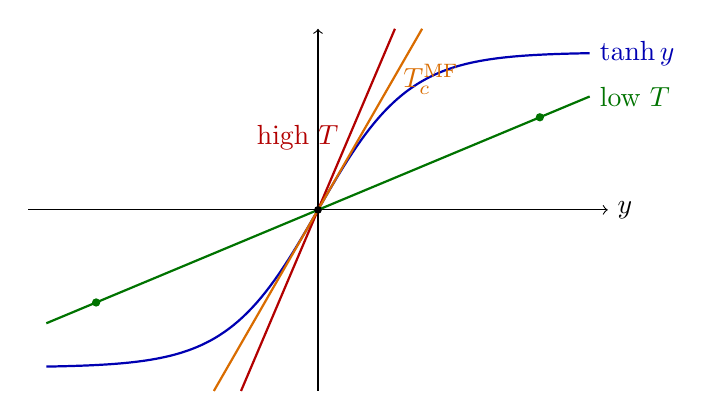
\begin{tikzpicture}[x=1.15cm,y=2.0cm]
\draw[->] (-3.2,0) -- (3.2,0) node[right] {$y$};
\draw[->] (0,-1.15) -- (0,1.15);
\draw[thick,blue!70!black,domain=-3:3,samples=120]
  plot (\x,{tanh(\x)}) node[right] {$\tanh y$};
\draw[thick,red!70!black] (-0.85,-1.15) -- (0.85,1.15)
  node[pos=0.70,left] {high \(T\)};
\draw[thick,orange!85!black] (-1.15,-1.15) -- (1.15,1.15)
  node[pos=0.86,right] {\(T_c^{\rm MF}\)};
\draw[thick,green!45!black] (-3,-0.72) -- (3,0.72)
  node[right] {low \(T\)};
\fill (0,0) circle (1.4pt);
\fill[green!45!black] (-2.45,-0.588) circle (1.5pt);
\fill[green!45!black] (2.45,0.588) circle (1.5pt);
\end{tikzpicture}
\caption{Một bản dựng lại đã chuẩn hóa của lập luận tự nhất quán bằng đồ thị.}
\end{figure}

Nhánh khác không xuất hiện liên tục. Gần điểm chuyển pha,
\begin{equation}
\tanh(Km)=Km-\frac{(Km)^3}{3}+O(m^5).
\end{equation}
Với \(K>1\), các nghiệm nhỏ khác không thỏa mãn
\begin{equation}
m^2\simeq \frac{3(K-1)}{K^3}.
\end{equation}
Vì vậy, lý thuyết trường trung bình dự đoán sự khởi phát dạng căn bậc hai quen thuộc \(m\propto(T_c-T)^{1/2}\).

Phát biểu về tính ổn định cũng có thể được nêu ra mà không cần dựa vào cách vẽ đồ thị. Bỏ qua một hằng số không phụ thuộc \(m\), năng lượng tự do trường trung bình trên mỗi spin là
\begin{equation}
f_{\rm MF}(m)
=dJm^2-\frac{1}{\beta}
\log\!\left[2\cosh(2\beta dJm)\right].
\label{eq:mf-free-energy}
\end{equation}
Điều kiện dừng của nó là
\begin{equation}
\frac{\partial f_{\rm MF}}{\partial m}
=2dJ\left[m-\tanh(2\beta dJm)\right]=0.
\end{equation}
Trên \(T_c^{\rm MF}\), \(m=0\) là cực tiểu. Bên dưới ngưỡng đó, gốc tọa độ là một cực đại địa phương và hai nghiệm khác không là các cực tiểu suy biến. Hình học của các giao điểm và nhiệt động học của năng lượng tự do nói cùng một điều.

\begin{classroomqa}
\audiencequestion{Nghiệm \(m=0\) vẫn còn là một giao điểm bên dưới \(T_c^{\rm MF}\). Vì sao nhánh khác không lại phải là nghiệm vật lý?}
\lecturerresponse{Khi đi theo hệ từ nhiệt độ không lên cao hơn, ta đã đặt nó trên một nhánh từ hóa. Nói hình thức hơn, bên dưới chuyển pha, năng lượng tự do trường trung bình có các cực tiểu tại \(\pm m_0\), còn \(m=0\) trở thành một cực đại. Khi đó, một trường ngoài vô cùng nhỏ sẽ chọn một cực tiểu và loại bỏ sự mơ hồ bề ngoài. \lecturetimestamp{01:11:34--01:12:18}}
\end{classroomqa}

\section{Vì sao một chiều làm trường trung bình thất bại}

Thế \(d=1\) vào Phương trình~\eqref{eq:mean-field-tc} sẽ dự đoán một chuyển pha tại \(T=2J\), mâu thuẫn với nghiệm chính xác một chiều. Không có biểu thức đại số nào phân kỳ. Gần đúng này thất bại vì hai láng giềng không phải là một bể thống kê lớn, và vì các vách miền một chiều mang một entropy đặc biệt lớn.

Xuất phát từ trạng thái tất cả spin đều hướng lên. Một liên kết bị phá vỡ làm năng lượng của nó đổi từ \(-J\) thành \(+J\), nên mỗi liên kết bị phá vỡ phải trả
\begin{equation}
\Delta E_{\rm bond}=2J.
\end{equation}
Trên mạng vuông, một spin lật làm đứt bốn liên kết và tốn \(8J\). Hai spin lật kề nhau có chu vi gồm sáu liên kết bị phá vỡ và tốn \(12J\), trong khi hai spin lật ở xa nhau phá vỡ tám liên kết và tốn \(16J\).

\begin{figure}[ht]
\centering
\includegraphics[width=0.82\textwidth]{lecture_09_figure_09.png}
\caption{Hai spin đảo chiều kề nhau trên một mạng vuông; liên kết chung của chúng vẫn được thỏa mãn, để lại một biên gồm sáu liên kết.}
\lectureframe{01:17:30}
\end{figure}

Vì vậy, trong hai chiều, một giọt miền đảo chiều gọn phải trả một năng lượng tỉ lệ với độ dài biên của nó:
\begin{equation}
\Delta E_{\rm 2d}=2J\,|\partial D|.
\end{equation}
Khi giọt ấy lớn lên thì nói chung biên của nó cũng lớn lên.

Một chiều thì khác. Một khối đảo chiều liên tiếp, dài đến đâu cũng vậy, chỉ có hai vách miền:
\begin{equation}
\Delta E_{\rm 1d}=2(2J)=4J.
\label{eq:one-d-domain-cost}
\end{equation}

\begin{figure}[ht]
\centering
\includegraphics[width=0.82\textwidth]{lecture_09_figure_10.png}
\caption{Một khối đảo chiều dài trong một chiều, chỉ được giới hạn bởi hai vách miền.}
\lectureframe{01:19:10}
\end{figure}

Có cỡ \(N^2\) cách để chọn hai vách của một khối như vậy trong một chuỗi gồm \(N\) vị trí. Năng lượng của chúng không tăng theo khoảng cách giữa hai vách. Vì thế, ở mọi nhiệt độ dương, entropy cho phép các miền đảo chiều lớn tùy ý. Trong hai chiều, ở nhiệt độ đủ thấp, năng lượng biên có thể thắng entropy đường bao. Sự cạnh tranh năng lượng-entropy này là sự kiện hình học mà trường trung bình không thể nhìn thấy khi nó chỉ coi \(d=1\) và \(d=2\) là những giá trị số khác nhau của cùng một hệ số.

\begin{classroomqa}
\audiencequestion{Chi phí không đổi của hai vách có đòi hỏi các spin bị lật phải kề nhau không?}
\lecturerresponse{Có. Mệnh đề này nói về một khối đảo chiều liên tiếp duy nhất. Nếu các spin bị lật tạo thành nhiều khối tách rời, mỗi khối sẽ đưa thêm hai vách miền nữa. Điểm quan trọng là một khối đơn lẻ có thể dài tùy ý mà vẫn chỉ giữ hai vách. \lecturetimestamp{01:18:32--01:18:40}}
\end{classroomqa}

\begin{classroomqa}
\audiencequestion{Bản thân phương trình trường trung bình dường như không cho thấy khác biệt định tính nào giữa \(d=1\) và \(d=2\). Có phải đó chính là vấn đề không?}
\lecturerresponse{Đúng vậy. Trường trung bình dự đoán một chuyển pha đối với mọi \(d\) dương, nên về mặt định tính nó sai trong một chiều. Phép suy ra của nó giả định có nhiều láng giềng dao động yếu và loại bỏ hình học của các vách miền. Trường hợp một chiều được quyết định bởi nghiệm chính xác theo liên kết, chứ không phải bởi phép thế trường trung bình \(d=1\). \lecturetimestamp{01:19:44--01:20:28}}
\end{classroomqa}

\section{Trường ngoài chọn pha}

Thêm một trường đều \(h\), với quy ước rằng \(h>0\) ưu tiên \(\sigma=+1\):
\begin{equation}
H=-J\sum_{\langle ij\rangle}\sigma_i\sigma_j
-h\sum_i\sigma_i.
\label{eq:ising-with-field}
\end{equation}
Năng lượng trường trung bình của một spin được chọn là
\begin{equation}
E_i^{\rm MF}=-(2dJm+h)\sigma_i,
\end{equation}
và phương trình tự hợp trở thành
\begin{equation}
\boxed{m=\tanh\!\left[\beta(2dJm+h)\right]}.
\label{eq:self-consistency-field}
\end{equation}
Với \(K=2\beta dJ\) và \(y=Km\),
\begin{equation}
\frac{y}{K}=\tanh(y+\beta h).
\label{eq:shifted-graph}
\end{equation}

\begin{figure}[ht]
\centering
\includegraphics[width=0.82\textwidth]{lecture_09_figure_11.png}
\caption{Hạng tử trường ngoài được thêm vào phương trình tự hợp, cùng với phép dựng đồ thị đã dịch chuyển.}
\lectureframe{01:26:20}
\end{figure}

\begin{classroomqa}
\audiencequestion{Vì sao trường chỉ được thêm vào bên trong hàm tang hyperbolic? Nó có nên làm thay đổi cả vế trái không?}
\lecturerresponse{Vế trái là độ từ hóa được giả định \(m\), hay tương đương là \(y/K\). Vế phải là độ từ hóa được tính cho một spin trong tổng trường hiệu dụng \(2dJm+h\). Tính tự hợp đặt hai đại lượng đó bằng nhau. Giữ \(y=Km\) cố định như định nghĩa sẽ đặt hạng tử mới chỉ vào đối số \(\tanh(y+\beta h)\). \lecturetimestamp{01:23:46--01:26:18}}
\end{classroomqa}

\begin{classroomqa}
\audiencequestion{Có thể mô tả cùng một thay đổi đồ thị bằng cách dịch chuyển các đường thẳng thay vì tịnh tiến đường cong \(\tanh\) không?}
\lecturerresponse{Có. Ta có thể giữ \(\tanh y\) cố định và viết lại phương trình sao cho đường thẳng có tung độ gốc khác không. Các giao điểm là y hệt nhau. Hai cách mô tả chỉ khác nhau ở việc chọn vế nào của phương trình làm đồ thị cố định. \lecturetimestamp{01:35:07--01:36:26}}
\end{classroomqa}

Với \(h\neq0\), gốc tọa độ không còn là một nghiệm. Bên dưới \(T_c^{\rm MF}\), một trường dương nhỏ tùy ý sẽ chọn nhánh dương; một trường âm sẽ chọn nhánh âm.

\begin{figure}[ht]
\centering
\includegraphics[width=0.82\textwidth]{lecture_09_figure_12.png}
\caption{Một trường yếu loại bỏ giao điểm đối xứng và chọn một nhánh từ hóa.}
\lectureframe{01:36:22}
\end{figure}

Phát biểu đúng đòi hỏi một thứ tự lấy giới hạn. Một hệ hữu hạn tại đúng \(h=0\) có đối xứng lật spin và vì thế \(\expect{m}=0\) trong toàn bộ ensemble cân bằng. Độ từ hóa tự phát là
\begin{equation}
m_{\rm sp}
=\lim_{h\to0^+}\lim_{N\to\infty}\expect{m}_{N,h},
\end{equation}
trong đó giới hạn nhiệt động học được lấy trước. Đảo dấu của trường vô cùng nhỏ cho \(-m_{\rm sp}\). Hiệu năng lượng trường toàn phần tỉ lệ với \(Nh\), nên ngay cả một trường rất nhỏ cũng trở nên có tính quyết định đối với một mẫu vĩ mô.

Năng lượng tự do tương ứng làm cho độ nghiêng trở nên rõ ràng:
\begin{equation}
f_{\rm MF}(m;h)
=dJm^2-\frac{1}{\beta}
\log\!\left[2\cosh\!\left(\beta(2dJm+h)\right)\right].
\end{equation}
Tại \(h=0\), hai giếng sâu như nhau. Một \(h\) dương hạ thấp giếng \(m\) dương và nâng cao giếng \(m\) âm. Nhiễu loạn trên mỗi spin có thể rất nhỏ, nhưng ưu thế tổng cộng sau khi nhân với \(N\) lại là vĩ mô.

\begin{classroomqa}
\audiencequestion{Nếu trường ngoài vẫn còn hiện diện, thì độ từ hóa đó có thật sự là tự phát không?}
\lecturerresponse{Trường chỉ được dùng để chọn một nhánh. Với \(T<T_c\) cố định, hãy lấy kích thước hệ ra vô hạn rồi sau đó cho \(h\to0^+\). Độ từ hóa vẫn hữu hạn dù trường chọn ấy triệt tiêu. Đảo dấu trong giới hạn sẽ chọn pha đối diện. \lecturetimestamp{01:33:15--01:34:18}}
\end{classroomqa}

\begin{classroomqa}
\audiencequestion{Nghiệm có trung bình bằng không bên dưới chuyển pha thật ra là bất khả, hay chỉ là không ổn định?}
\lecturerresponse{Ở trường đúng bằng không, một ensemble đối xứng trong thể tích hữu hạn với trọng số bằng nhau cho hai hướng là khả dĩ và có trung bình bằng không. Điều thất bại là tính ổn định của nó như một pha vĩ mô đơn lẻ. Một trường nhỏ tùy ý làm thay đổi cân bằng năng lượng quảng tính và chọn một hướng; sau giới hạn nhiệt động học, độ từ hóa đã được chọn vẫn còn lại khi trường bị loại bỏ. \lecturetimestamp{01:34:25--01:35:06}}
\end{classroomqa}

\begin{classroomqa}
\audiencequestion{Điều gì xảy ra với nghiệm bị trường thiên lệch ở nhiệt độ vô hạn?}
\lecturerresponse{Với \(h\) hữu hạn cố định, cả \(K=2\beta dJ\) lẫn \(\beta h\) đều triệt tiêu khi \(T\to\infty\). Khi đó, Phương trình~\eqref{eq:self-consistency-field} cho \(m\to0\). Trường yếu chọn một nhánh ở nhiệt độ thấp, nhưng nó không thể duy trì trật tự trước sự khuấy động nhiệt vô hạn. \lecturetimestamp{01:27:39--01:29:51}}
\end{classroomqa}

\begin{classroomqa}
\audiencequestion{Khi nhiệt độ và độ dịch của đồ thị cùng thay đổi, làm sao có thể chắc được giao điểm đi về đâu?}
\lecturerresponse{Phương trình ẩn an toàn hơn hình phác đang dịch chuyển. Ở nhiệt độ thấp và \(h\) dương, nghiệm ổn định của nó tiến tới \(m=+1\). Ở nhiệt độ cao, khai triển hàm tang cho
\[
m\simeq \beta(2dJm+h)
\quad\Longrightarrow\quad
m\simeq \frac{\beta h}{1-2\beta dJ},
\]
đại lượng này tiến về không khi \(\beta\to0\). Vì thế, nhánh ổn định nối giới hạn nhiệt độ thấp thẳng hàng với giới hạn nhiệt độ cao phân cực yếu mà không ở lại tại gốc không ổn định bên dưới chuyển pha. \lecturetimestamp{01:29:53--01:33:04}}
\end{classroomqa}

\section{Sự đảo chiều từ hóa là một bài toán khác}

\begin{classroomqa}
\audiencequestion{Điều gì làm cho từ trường Trái Đất đảo ngược hướng?}
\lecturerresponse{Câu hỏi đó nằm ngoài mô hình Ising cân bằng. Từ trường chính của Trái Đất được tạo ra bởi geodynamo: sự đối lưu và sự quay của chất lưu dẫn điện trong lõi ngoài duy trì các dòng điện và từ trường. Các lần đảo chiều là những sự tái tổ chức bất quy tắc của dynamo phi tuyến ấy, chứ không phải một sự lật miền sắt từ đơn giản trong sắt rắn. Thời điểm chi tiết của chúng không được mô tả bởi một tham số trật tự cân bằng duy nhất, vì vậy câu trả lời thẳng thắn ở đây là phép tính Ising không giải thích được yếu tố kích hoạt. Mối liên hệ hữu ích chỉ là ở mức tổng quát: một hệ có hai định hướng vĩ mô đối nghịch có thể trải qua một bất ổn định giữa hai định hướng ấy.\footnote{Xem \href{https://science.nasa.gov/science-research/earth-science/earths-magnetosphere-protecting-our-planet-from-harmful-space-energy/}{bài tổng quan của NASA về geodynamo} và \href{https://www.usgs.gov/programs/geomagnetism/introduction-geomagnetism}{phần giới thiệu của USGS về địa từ học}.} \lecturetimestamp{01:38:39--01:40:32}}
\end{classroomqa}

Chuỗi được giải chính xác và mạng trường trung bình giờ đây cho hai câu trả lời khác nhau rõ rệt. Trong một chiều,
\begin{equation}
\expect{\sigma_i\sigma_{i+r}}
=\left[\tanh(\beta J)\right]^r
\longrightarrow0
\qquad (T>0),
\end{equation}
vì các vách miền có năng lượng hữu hạn có thể ngăn cách những đoạn bị đảo ngược dài tùy ý. Ngược lại, với nhiều láng giềng, trường tự hợp thừa nhận các nghiệm ổn định khác không khi nhiệt độ thấp hơn
\begin{equation}
T_c^{\rm MF}=2dJ.
\end{equation}
Sự tương phản này không chỉ đơn thuần là đại số. Đó là sự cạnh tranh giữa hình học, năng lượng, entropy và tính dư thừa: liệu một lỗi có thể lan truyền tự do hay mạng xung quanh có thể sửa nó.